\subsection*{Solution to Spring 2014, \#1}\label{s141}
This problem is similar to Evans, Page 87, Problem \#15.
Let $u$ be a solution to the PDE. Let $v(x, t) := e^{t}u(x, t)$. Then
$v_{t} = e^{t}u + e^{t}u_{t}$ and $v_{xx} = e^{t}u_{xx}$. Thus
$$0 = u_{t} - u_{xx} + u = e^{-t}v_{t} - e^{-t}v - e^{-t}v_{xx} + e^{-t}v = e^{-t}(v_{t} - v_{xx}).$$
Therefore
\begin{align*}
\begin{cases}
v_{t} - v_{xx}  = 0 & \text{ for } x > 0, t > 0\\
v(x, 0) = f(x) &\text{ for } x > 0\\
v(0, t) = e^{t}g(t) & \text{ for } t > 0.
\end{cases}
\end{align*}
Note that $f, g$ are compactly supported in $(0, \infty)$ and hence $f(0) = 0$, $g(0) = 0$ and $f, g$ vanish in some sufficiently
small neighborhood of $0$.

Let $w(x, t) := v(x, t) - f(x) - e^{t}g(t)$. Then
$$w(x, 0) = v(x, 0) - f(x) - g(0) = 0$$
for $x > 0$, $$w(0, t) = v(0, t) - f(0) - e^{t}g(t) = 0$$ for $t > 0$, and
$$w_{t} - w_{xx} = v_{t} - (e^{t}g(t))' - v_{xx} + f''(x) = f''(x) - e^{t}(g(t) + g'(t))$$
for $x > 0$, $t > 0$.
That is,
\begin{align*}
\begin{cases}
w_{t} - w_{xx} = f''(x) - e^{t}(g(t) + g'(t)) & \text{ for } x > 0, t > 0\\
w(x, 0) = 0 & \text{ for } x > 0\\
w(0, t) = 0 & \text{ for } t > 0.
\end{cases}
\end{align*}
Since $f, g$ are compactly supported in $(0, \infty)$, $f''(x) - e^{t}(g(t) + g'(t))$ vanishes
in a neighborhood of $(0, 0)$. We extend $w$ to the negative $x$-axis by odd reflection.
That is, let
\begin{align*}
\wt{w}(x, t) =
\begin{cases}
w(x, t) & \text{ if } x \geq 0, t \geq 0\\
-w(-x, t) & \text{ if } x \leq 0, t \geq 0.
\end{cases}
\end{align*}
Then if $x > 0$ and $t > 0$,
$\wt{w}_{t} - \wt{w}_{xx} = f''(x) - e^{t}(g(t) + g'(t))$. If $x < 0$ and $t > 0$, then
\begin{align*}
\wt{w}_{t} - \wt{w}_{xx} &= \frac{\pr}{\pr t}(-w(-x, t)) - \frac{\pr^{2}}{\pr x^{2}}(-w(-x, t))\\
& = -w_{t}(-x, t) + w_{xx}(-x, t) = -f''(-x) + e^{t}(g(t) + g'(t)).
\end{align*}
Furthermore, for $x \in \R$,
\begin{align*}
\wt{w}(x, 0) =
\begin{cases}
w(x, 0) & \text{ if } x \geq 0\\
-w(-x, 0) & \text{ if } x \leq 0
\end{cases} = 0
\end{align*}
and $\wt{w}(0, t) = 0$ for $t \geq 0$.
Let
\begin{align*}
h(x, t) :=
\begin{cases}
f''(x) - e^{t}(g(t) + g'(t)) & \text{ if } x > 0, t > 0\\
-f''(-x) + e^{t}(g(t) + g'(t)) & \text{ if } x < 0, t > 0.
\end{cases}
\end{align*}
Thus $\wt{w}$ satisfies the following non-homogenous heat equation in $\R$:
\begin{align*}
\begin{cases}
\wt{w}_{t} - \wt{w}_{xx} =h(x, t) & \text{ if } x \in \R, t > 0\\
\wt{w}(x, 0) = 0 & \text{ if } x \in \R\\
\wt{w}(0, t) = 0 & \text{ if } t \geq 0.
\end{cases}
\end{align*}
Let $\Phi(x, t) := \frac{1}{\sqrt{4\pi t}}e^{-x^{2}/(4t)}1_{t > 0}.$ Then
\begin{align*}
\wt{w}(x, t) &= \int_{0}^{t}\int_{-\infty}^{0}\Phi(x - y, t - s)(-f''(-y) + e^{s}(g(s) + g'(s)))\, dy\, ds\\
&\quad\quad + \int_{0}^{t}\int_{0}^{\infty}\Phi(x - y, t - s)(f''(y) - e^{s}(g(s) + g'(s)))\, dy\, ds.
\end{align*}
Therefore a solution $u$ is given by
$$u(x, t) = e^{-t}(\wt{w}(x, t) + f(x) + e^{t}g(t)) = e^{-t}\wt{w}(x, t) + e^{-t}f(x) + g(t)$$
for $x > 0$, $t > 0$.
\hfill\qed

\subsection*{Solution to Spring 2014, \# 2}\label{s142}
This problem will utilize what we call the ``$L^{p}$ trick." The moral is that if we are on space with finite measure (for example a bounded open set),
to control behavior about the supremum of a function, it is enough to control behavior of the $L^{p}$ norm of this function and then pass to the limit.
\subsubsection*{Solution to $2a$}
Let $w := u_{1} - u_{2}$. Then
\begin{equation*}
\begin{cases}
w_{t} - \Delta w = 0 & \text{ in } \Om \times (0, \infty)\\
\pr w/\pr \nu = 0 & \text{ on } \pr\Om \times (0, \infty).
\end{cases}
\end{equation*}
Note that $A(t) = \nms{w}_{L_{x}^{\infty}(\Om)}$. We will emphasize the dependence of $\nms{w}_{L_{x}^{p}(\Om)}$ (for any $p$) on $t$ by writing
$\nms{w(t)}$ in place of $\nms{w}$. Since $\Om$ is a bounded open set, it has finite measure. Then
\begin{align}\label{s142aeq1}
\nms{w(t)}_{L_{x}^{\infty}(\Om)} = \lim_{p \rightarrow \infty}\nms{w(t)}_{L_{x}^{p}(\Om)} = \lim_{p \rightarrow \infty}\left(\int_{\Om}|w(x, t)|^{p}\, dx\right)^{1/p}.
\end{align}
We want to show that if $t_{1} \geq t_{2}$, then $A(t_{1}) \leq A(t_{2})$. For $p \geq 2$, let $\psi(x) := \abn{x}^{p}$. Note that $\psi \in C^{2}$ for $p \geq 2$.
Since
\begin{align*}
\frac{\pr}{\pr t}\int_{\Om}\psi(w)\, dx &= \int_{\Om}\psi'(w) w_{t}\, dx = \int_{\Om}\psi'(w)\Delta w\, dx\\
& = -\int_{\Om}\nabla(\psi'(w))\cdot \nabla w\, dx = -\int_{\Om}\psi''(w)\sum_{i = 1}^{n}w_{x_{i}}^{2}\, dx \leq 0
\end{align*}
where the third equality is because $\pr w/\pr\nu = 0$ and the last inequality is because $\psi'' \geq 0$ (since $\psi$ is concave up).
Therefore for each $p \geq 2$, $\int_{\Om}|w(x, t)|^{p}\, dx$ is monotonically decreasing as a function of $t$ and hence so is $\nms{w(t)}_{L^{p}_{x}(\Om)}$.
Combining this with \eqref{s142aeq1} yields that for $t_{1} \geq t_{2}$,
\begin{align*}
A(t_{1}) = \nms{w(t_{1})}_{L_{x}^{\infty}(\Om)} &= \lim_{p \rightarrow \infty}\left(\int_{\Om}|w(x,t_{1})|^{p}\right)^{1/p} \\
&\leq \lim_{p \rightarrow \infty}\left(\int_{\Om}|w(x,t_{2})|^{p}\right)^{1/p} =\nms{w(t_{2})}_{L_{x}^{\infty}(\Om)} = A(t_{2}).
\end{align*}
Since $t_{1}$ and $t_{2}$ were arbitrary, it follows that $A(t)$ decreases in time.
\hfill\qed

\subsubsection*{Solution to $2b$}
There seems to be a typographical error in the statement of this problem. If this problem was true, then
for sufficiently large $t$, $\pr_{\nu}u_{1} = \nabla u_{1} \cdot \nu$ should be fairly close to $0$ but this can be potentially very
far away from the value of $f$.

Assume $u_{1}$ and $u_{2}$ are both uniformly $C^{2}$ in space and time. Then by the above calculation
\begin{align*}
0 \leq A(t) &= \nms{w(t)}_{L_{x}^{\infty}(\Om)} = \lim_{p \rightarrow \infty}\nms{w(t)}_{L_{x}^{p}(\Om)}\\
 &\leq \lim_{p \rightarrow \infty}\nms{w(0)}_{L_{x}^{p}(\Om)} = \nms{w(0)}_{L_{x}^{\infty}(\Om)} = \nms{w(x, 0)}_{L_{x}^{\infty}} < \infty
\end{align*}
where the second inequality is because $\nms{w(t)}_{L_{x}^{p}(\Om)}$ is decreasing in time for each $p$
and $\nms{w(x, 0)}_{L_{x}^{\infty}}$ is finite since $u_{1}$ and $u_{2}$ are uniformly $C^{2}$ in both variables. Combining this with part $(a)$ yields that there exists
a constant $C$ such that $A(t) \rightarrow C$ as $t \rightarrow \infty$, however, this does not imply that either $u_{1}$ or $u_{2}$ converge to a constant
as $t \rightarrow \infty$.
\hfill\qed

\subsection*{Solution to Spring 2014, \#3}\label{s143}
\subsubsection*{Solution to $3a$}
For a function $f: \mathbb{R}^{n} \rightarrow \R$, we will use the following convention for the Fourier transform, we define
$$\wh{f}(\xi) = \frac{1}{(2\pi)^{n/2}}\int_{\R^{n}}f(x)e^{-ix\cdot \xi}\, dx.$$
Since $D_{1}$ is positive definite, it is invertible and hence let $M := D_{1}^{-1}D_{2}$. Thus we want to solve
$$\mb{v}_{t} + M\mb{v}_{x} = 0.$$
Taking the Fourier transform of both sides yields that
\begin{align}\label{s143aeq1}
(\wh{\mb{v}})_{t} + i\xi M\wh{\mb{v}} = 0
\end{align}
where $\wh{\mb{v}}(\xi, t) = (\wh{v_{1}}(\xi, t), \ldots, \wh{v_{n}}(\xi, t))$. Rearranging and solving for $\wh{\mb{v}}$ in \eqref{s143aeq1}
yields that
$$\wh{\mb{v}}(\xi, t) = \wh{\mb{v}}(\xi, 0)\exp(-i\xi M)$$
where $\exp$ here is the matrix exponential and $\wh{\mb{v}}(\xi, 0)$ is the Fourier transform
of $v(x, 0)$. Taking the Fourier inverse of both sides yields that the solution is
$$\mb{v}(x, t) = [\wh{\mb{v}}(\xi, 0)\exp(-i\xi M)]^{v} = [\wh{\mb{v}}(\xi, 0)\exp(-i\xi D_{1}^{-1}D_{2})]^{v}.$$
\hfill\qed

\subsubsection*{Solution to $3b$}
The Fourier transform approach in part $(a)$ will still apply in this case. However, we illustrate a linear algebra approach.
We first prove the following linear algebra lemma.
\begin{lemma}\label{s143blem1}
If $A$ and $B$ are symmetric matrices and $A$ is positive definite, then $AB$ is diagonalizable.
\end{lemma}
\begin{proof}
% http://pages.cs.wisc.edu/~yanchao/LinearAlgebraFactSheet.pdf
Since $A$ is positive definite, there exists a symmetric invertible matrix $Q$ such that $Q^{2} = A$.
Then $Q^{-1}ABQ = QBQ$. Since $(QBQ)^{t} = Q^{t}(QB)^{t} = Q^{t}B^{t}Q^{t} = QBQ$, $QBQ$ is symmetric and
hence $AB$ is similar to a symmetric matrix. Since symmetric matrices are diagonalizable, $AB$ is diagonalizable.
This completes the proof of Lemma \ref{s143blem1}.
\end{proof}
Since $D_{1}$ is positive definite, it is invertible and hence we want to solve
\begin{align}\label{s143beq1}
\mb{v}_{t} + D_{1}^{-1}D_{2}\mb{v}_{x} = 0
\end{align}
where $\mb{v} = (v_{1}, \ldots, v_{n})^{t}$.
Since $D_{1}$ is positive definite, so is $D_{1}^{-1}$ and hence by Lemma \ref{s143blem1},
$D_{1}^{-1}D_{2}$ is diagonalizable. That is, there an invertible matrix $P$ and a diagonal matrix $\Ld$ such that
\begin{align}\label{s14pdef}
D_{1}^{-1}D_{2} = P^{-1}\Ld P.
\end{align}
Let $\mb{w} := P\mb{v}$. Then \eqref{s143beq1} becomes
\begin{align*}
(P^{-1}\mb{w})_{t} + P^{-1}\Ld P(P^{-1}\mb{w})_{x} = 0
\end{align*}
and as $P^{-1}$ is invertible, we have
$$\mb{w}_{t} + \Ld \mb{w}_{x} = 0.$$
Writing $\mb{w} = (w_{1}, \ldots, w_{n})^{t}$ and letting $\Ld = \textrm{diag}(\ld_{1}, \ldots, \ld_{n})$, the above PDE decouples
into $n$ disjoint transport equations of the form
\begin{align}\label{s143beq2}
(w_{i})_{t} = \ld_{i}(w_{i})_{x}, \quad i = 1, 2, \ldots, n.
\end{align}
Let $G_{i}(x) := w_{i}(x, 0)$ be the $i$th row of the column vector
\begin{align}\label{s14pfmat}
P\mb{v}(x, 0) = P\begin{pmatrix}
v_{1}(x, 0)\\
v_{2}(x, 0)\\
\vdots\\
v_{n}(x, 0)
\end{pmatrix}.
\end{align}
Therefore the solution to \eqref{s143beq2} is $$w_{i}(x, t) = G_{i}(x + \ld_{i}t) = w_{i}(x + \ld_{i}t, 0).$$ Since $\mb{v} = P^{-1}\mb{w}$,
it follows that
\begin{align*}
\mb{v} = \begin{pmatrix}
v_{1}(x, t)\\
v_{2}(x, t)\\
\vdots\\
v_{n}(x, t)
\end{pmatrix}=
P^{-1}
\begin{pmatrix}
w_{1}(x, t)\\
w_{2}(x, t)\\
\vdots\\
w_{n}(x, t)
\end{pmatrix}=
P^{-1}
\begin{pmatrix}
w_{1}(x + \ld_{1}t, 0)\\
w_{2}(x + \ld_{2}t, 0)\\
\vdots\\
w_{n}(x + \ld_{n}t, 0)
\end{pmatrix}
\end{align*}
where $P$ is defined as in \eqref{s14pdef}, the $\ld_{i}$ are the eigenvalues of the matrix $D_{1}^{-1}D_{2}$, and $w_{i}$ is the $i$-th row of \eqref{s14pfmat}.
\hfill\qed

\subsection*{Solution to Spring 2014, \#4}\label{s144}

\subsubsection*{Solution to 4a}

With $n=1$, the eikonal equation reads
\[
u_t + \frac{1}{2} (u_x)^2 = 0 \,\, \text{in} \,\, (x,t) \in \R \times (0,\infty)
\]
with initial data $u(x,0) = -x^2$. We can solve this using method of characteristics. Define
\[
F(x,t,z,p,q) = q + \frac{1}{2}p^2
\]
where $z := u$, $q := u_t$, and $p := u_x$. Then, the ODEs that we must solve are as follows:
\begin{equation}
\label{s14one} \dot t(s) = 1, \quad t(0) = 0
\end{equation}
\begin{equation}
\label{s14two}
\dot x(s) = p(s), \quad x(0) = x_0
\end{equation}
\begin{equation}
\label{s14three}
\dot z(s) = q(s) + p(s)^2, \quad z(0) = -x_0^2
\end{equation}
\begin{equation}
\label{s14four}
\dot p(s) = 0, \quad p(0) = -2x_0
\end{equation}
\begin{equation}
\label{s14five}
\dot q(s) = 0, \quad q(0) = -2x_0^2
\end{equation}
Solving \eqref{s14one}, \eqref{s14four}, and \eqref{s14five} yield
\[
t(s) = s, \quad \quad p(s) = -2x_0, \quad \quad q(s) = -2x_0^2
\]
respectively. Then, solving \eqref{s14two} and \eqref{s14three} yield
\[
x(s) = -2x_0 s + x_0, \quad \quad z(s) = 2x_0^2 s - x_0^2
\]
There are now two ways for us to reach the desired conclusion: by examining the characteristics, or by finding the explicit solution. Both approaches are discussed.

\vspace{0.4cm}

From solving \eqref{s14two}, we find that the characteristics are $x_{x_0}(t) = x_0 (1-2t)$ for $x_0 \in \R$, where the subscript $x_0$ implies that the characteristic starts at $x_0$. Observe that, for any $x_0$, $x_{x_0}(1/2) = 0$, implying that all of the characteristics crash at $t=1/2$. Therefore, we don't expect a smooth solution.

\vspace{0.4cm}

To find the explicit solution, we solve for $x_0$ in terms of $x$ and $t$, which gives us
\[
x_0 = \frac{x}{1-2t}
\]
Hence,
\[
u(x,t) = 2\left(\frac{x}{1-2t} \right)^2 t - \left( \frac{x}{1-2t} \right)^2 = \frac{x^2}{2t-1}
\]
and we see that $u(x,t)$ blows up as $t$ approaches $1/2$. Therefore, the solution isn't smooth.  \qed

\subsubsection*{Solution to 4b}

For $n>2$, the eikonal equation reads
\[
u_t + \frac{1}{2} |\del u|^2 = 0 \,\, \text{in} \,\, (x,t) \in \R^n \times (0, \infty)
\]
with initial data $u(x,0) = -|\vx|^2$. Again, we use the method of characteristics. Define
\[
F(\vx,t,z,\vp,q) = q + \frac{1}{2}|\vp|^2
\]
where $z:=u$, $q:=u_t$, and $\vp:=\del u$. Then, the ODEs that we must solve are as follows:
\begin{equation}
	\label{s14six}
	\dot t(s) = 1, \quad t(0) = 0	
\end{equation}
\begin{equation}
	\label{s14seven}
	\dot \vx(s) = \vp(s), \quad \vx(0) = \vx_0
\end{equation}
\begin{equation}
	\label{s14eight}
	\dot z(s) = q(s) + |\vp(s)|^2, \quad z(0) = -|\vx_0|^2
\end{equation}
\begin{equation}
	\label{s14nine}
	\dot \vp(s) = 0, \quad \vp(0)=-2\vx_0
\end{equation}
\begin{equation}
	\label{s14ten}
	\dot q(s) = 0, \quad q(0) = -2|\vx_0|^2
\end{equation}
Solving \eqref{s14six}, \eqref{s14nine}, and \eqref{s14ten} yield
\[
t(s) = s, \quad \vp(s) = -2\vx_0, \quad q(s) = -2|\vx_0|^2
\]
respectively. Then, solving \eqref{s14seven} and \eqref{s14eight} yield
\[
\vx(s) = -2\vx_0 s + \vx_0, \quad z(s) = 2|\vx_0|^2 s + |\vx_0|^2
\]
Solving for $\vx_0$ in terms of $\vx$ and $t$ yields
\[
\vx_0 = \frac{\vx}{1-2t}
\]
which implies
\[
u(\vx,t) = \frac{|\vx|^2}{2t-1}
\]
Again, the solution blows up as $t$ approaches $1/2$, so the solution isn't smooth. \hfill\qed

\subsection*{Solution to Spring 2014, \#5}\label{s145}
\begin{rem}
We correct a few significant typographical errors that occur in the problem statement. First, since we are seeking solutions to the Euler-Bernouilli equation
of the form $w(x, t) = u(x)e^{i\om t}$ (to avoid confusion we will use $u$ and $\om$ rather than $w$ and $\om$ as in the problem statement), then
$$\rho u(x)(i\om)^{2}e^{i\om t} = -EIu^{(4)}(x)e^{i\om t}$$
and hence
\begin{align}\label{s14first}
EI\frac{d^{4}u}{dx^{4}} = \rho\om^{2} u
\end{align}
this change will play a significant role in calculating the lowest normal frequency (otherwise as stated, running through the (tedious) argument would give that $\om$ is imaginary).

Next, denote $D$ the differential operator defined by $Df := EI(d^4f/dx^{4})$. To ensure that $D$ is self-adjoint, we need the boundary conditions
$$u''(L) = 0 \quad \text{ and } \quad u'''(L) = 0$$
rather than $u'''(L) = 0$ and $u''''(L) = 0$. With these changes, we solve the problem. \hfill\qed
\end{rem}

\subsubsection*{Solution to $5a$}
The wording for this problem is derived from Chapter 7, Section 2-3 of Coddington and Levinson. For a reference for the discussion below, see Page 192 of that book.
The Green's function for the eigenequation (or more precisely the Green's function for the eigenvalue problem) is a function $\wt{G}(x, \xi, \om)$ such that the solution
to
\begin{align}\label{s14main}
EI\frac{d^{4}u}{dx^{4}} - \rho\om^{2}u = f
\end{align}
with $u(0) = 0, u'(0) = 0, u''(L) = 0, u'''(L) = 0$ is given by
$$u(x) = \int_{0}^{L}\wt{G}(x, \xi, \om)f(\xi)\, d\xi.$$
We will find the Green's function $G(x, \xi, \om)$ for the problem
$$\frac{d^{4}u}{dx^{4}} - \frac{\rho\om^{2}}{EI}u = f$$
with $u(0) = 0, u'(0) = 0, u''(L) = 0, u'''(L) = 0$. Then
\begin{align}\label{s14green_rel}
\wt{G}(x, \xi, \om) = \frac{1}{EI}G(x, \xi, \om).
\end{align}
We will split into two cases, when $\om = 0$ and when $\om \neq 0$.

We first consider the $\om = 0$ case. Then we want to find the Green's function for
$$\frac{d^{4}u}{dx^{4}} = f$$
with $u(0) = 0$, $u'(0) = 0$, $u''(L) = 0$, and $u'''(L) = 0$. Let $G(x, \xi)$ with $\xi \in [0, L]$ denote the Green's function
in this case (this is slight abuse of notation, but $G(x, \xi) = G(x, \xi, 0)$). Then $G(x, \xi)$ is a function
such that
$$\frac{d^{4}}{dx^{4}}G(x, \xi) = \delta(x - \xi)$$
with $G(0, \xi) = 0$, $G'(0, \xi) = 0$, $G''(L, \xi) = 0$, and $G'''(L, \xi) = 0$.
The set $\{1, x, x^{2}, x^{3}\}$ forms a fundamental set of solutions for the homogenous problem.

Let $y_{1} := 1$, $y_{2} := x$, $y_{3} := x^{2}$, and $y_{4} := x^{3}$ and let $B_{i}, i = 1, 2, 3, 4$ act on functions $f$ as follows:
$B_{1}[f] = f(0)$, $B_{2}[f] = f'(0)$, $B_{3}[f] = f''(L)$, and $B_{4}[f] = f'''(L)$. Then the Green's function is given by
$$G(x, \xi) = 1_{x > \xi}y_{\xi}(x) + \sum_{j = 1}^{4}a_{j}y_{j}(x)$$
where $y_{\xi}$ is a linear combination of the $\{y_{i}\}$ such that
$$y_{\xi}(\xi) = 0, \,\,\, y_{\xi}'(\xi) = 0, \,\,\, y_{\xi}''(\xi) = 0, \,\,\,y_{\xi}'''(\xi) = 1.$$
and $a_{1}, a_{2}, a_{3}, a_{4}$ are such that
\begin{align}\label{s14amat}
\begin{pmatrix}
B_{1}[y_1] & B_{1}[y_2] & B_{1}[y_3] & B_{1}[y_4]\\
B_{2}[y_1] & B_{2}[y_2] & B_{2}[y_3] & B_{2}[y_4]\\
B_{3}[y_1] & B_{3}[y_2] & B_{3}[y_3] & B_{3}[y_4]\\
B_{4}[y_1] & B_{4}[y_2] & B_{4}[y_3] & B_{4}[y_4]
\end{pmatrix}
\begin{pmatrix}
a_1\\ a_2 \\ a_3\\ a_4
\end{pmatrix}
=
\begin{pmatrix}
-B_{1}[1_{\cdot > \xi}y_{\xi}(\cdot)]\\
-B_{2}[1_{\cdot > \xi}y_{\xi}(\cdot)]\\
-B_{3}[1_{\cdot > \xi}y_{\xi}(\cdot)]\\
-B_{4}[1_{\cdot > \xi}y_{\xi}(\cdot)]
\end{pmatrix}
\end{align}
We now compute $y_{\xi}$. Let $y_{\xi}(x) = a + bx + cx^{2} + dx^{3}$ and we compute $a, b, c, d$.
Since we want $y_{\xi}(\xi) = 0$, $y_{\xi}'(\xi) = 0$, $y_{\xi}''(\xi) = 0$, and $y_{\xi}'''(\xi) = 1$,
we obtain the following system
\begin{align*}
a + b\xi + c\xi^{2} + d\xi^{3} & = 0\\
b + 2c\xi + 3d\xi^{2} & = 0\\
2c + 6d\xi &= 0\\
6d & = 1
\end{align*}
and hence $a = -(1/6)\xi^{3}$, $b = (1/2)\xi^{2}$, $c = -\xi/2$, and $d = 1/6$.
Therefore
$$y_{\xi}(x) = -\frac{1}{6}\xi^{3} + \frac{1}{2}\xi^{2}x - \frac{1}{2}\xi x^{2} + \frac{1}{6}x^{3} = \frac{1}{6}(x- \xi)^{3}.$$
We now compute $a_{1}, a_{2}, a_{3}, a_{4}$ in \eqref{s14amat}.
We have
\begin{align*}
\begin{pmatrix}
B_{1}[y_1] & B_{1}[y_2] & B_{1}[y_3] & B_{1}[y_4]\\
B_{2}[y_1] & B_{2}[y_2] & B_{2}[y_3] & B_{2}[y_4]\\
B_{3}[y_1] & B_{3}[y_2] & B_{3}[y_3] & B_{3}[y_4]\\
B_{4}[y_1] & B_{4}[y_2] & B_{4}[y_3] & B_{4}[y_4]
\end{pmatrix} =
\begin{pmatrix}
1 & 0 & 0 & 0\\
0 & 1 & 0 & 0\\
0 & 0 & 2 & 6L\\
0 & 0 & 0 & 6
\end{pmatrix}.
\end{align*}
Since
\begin{equation*}
1_{x > \xi}y_{\xi}(x) =
\begin{cases}
\frac{1}{6}(x- \xi)^{3} & \text{if } x > \xi\\
0 & \text{otherwise,}
\end{cases}
\end{equation*}
it follows that
\begin{align*}
a_{1} &= -B_{1}[1_{\cdot > \xi}y_{\xi}(\cdot)] = 0\\
a_{2} &= -B_{2}[1_{\cdot > \xi}y_{\xi}(\cdot)] = 0\\
a_{4} &= -\frac{1}{6}B_{4}[1_{\cdot > \xi}y_{\xi}(\cdot)] = -\frac{1}{6}
\end{align*}
and $$2a_{3} + 6La_{4} = -B_{3}[1_{\cdot > \xi}y_{\xi}(\cdot)] = -(L - \xi)$$ which implies that
$$a_{3} = \xi/2$$
This implies that the Green's function in the case of $\om = 0$ is
\begin{align*}
G(x, \xi, 0) = G(x, \xi) = 1_{x > \xi}\frac{1}{6}(x - \xi)^{3} + \frac{\xi}{2}x^{2} - \frac{1}{6}x^{3}
\end{align*}
which by \eqref{s14green_rel} implies that the Green's function in the case of $\om = 0$ to \eqref{s14main} is
\begin{align}\label{s14green}
\wt{G}(x, \xi, 0) = \frac{1}{EI}(1_{x > \xi}\frac{1}{6}(x - \xi)^{3} + \frac{\xi}{2}x^{2} - \frac{1}{6}x^{3}).
\end{align}

We now consider the $\om \neq 0$ case. We will follow the same method as in the $\om = 0$ case.
Fix an $\om \neq 0$, we want to find a Green's function for $$\frac{d^{4}u}{dx^{4}} - \frac{\rho\om^{2}}{EI}u = f$$
with $u(0) = 0, u'(0) = 0, u''(L) = 0, u'''(L) = 0$.
Let $\beta := (\frac{\rho\om^{2}}{EI})^{1/4}$ and let $y_{1} := e^{\beta x}$, $y_{2} := e^{-\beta x}$, $y_{3} := \cos(\beta x)$,
and $y_{4} := \sin (\beta x)$. The $\{y_{i}\}$ once again form a fundamental set of solutions for the homogenous problem. Let
the functionals $B_{i}$ be defined as in the $\om = 0$ case. We first compute $$y_{\xi} = ay_{1} + by_{2} + cy_{3} + dy_{4}$$
by finding $a, b, c, d$. Since we want $y_{\xi}(\xi) = 0$, $y_{\xi}'(\xi) = 0$, $y_{\xi}''(\xi) = 0$, and $y_{\xi}'''(\xi) = 1$,
we obtain the following system
\begin{align}\label{s14abcd}
\begin{pmatrix}
e^{\beta\xi} & e^{-\beta\xi} & \cos(\beta \xi) & \sin(\beta \xi)\\
\beta e^{\beta \xi} & -\beta e^{-\beta \xi} & -\beta \sin(\beta \xi) & \beta \cos(\beta \xi)\\
\beta^{2}e^{\beta \xi} & \beta^{2}e^{-\beta \xi} & -\beta^{2}\cos(\beta \xi) & -\beta^{2}\sin(\beta \xi)\\
\beta^{3}e^{\beta \xi} & -\beta^{3}e^{-\beta \xi} & \beta^{3}\sin(\beta \xi) & -\beta^{3}\cos(\beta \xi)
\end{pmatrix}
\begin{pmatrix}
a\\b\\c\\d
\end{pmatrix}
=
\begin{pmatrix}
0\\0\\0\\1
\end{pmatrix}.
\end{align}
Inverting the matrix on the left would yield the desired $a, b, c, d$ to construct $y_{\xi}(x)$.
Now we find $a_{1}, a_{2}, a_{3}, a_{4}$ as in \eqref{s14amat}. We want to solve
\begin{align*}
\begin{pmatrix}
1 & 1 & 1 & 0\\
\beta & -\beta & 0 & \beta\\
\beta^{2}e^{\beta L} & \beta^{2}e^{-\beta L} & -\beta^{2}\cos(\beta L) & -\beta^{2}\sin(\beta L)\\
\beta^{3}e^{\beta L} & -\beta^{3}e^{-\beta L} & \beta^{3}\sin(\beta L) & -\beta^{3}\cos(\beta L)
\end{pmatrix}
\begin{pmatrix}
a_1\\ a_2 \\ a_3\\ a_4
\end{pmatrix}
=
\begin{pmatrix}
-B_{1}[1_{\cdot > \xi}y_{\xi}(\cdot)]\\
-B_{2}[1_{\cdot > \xi}y_{\xi}(\cdot)]\\
-B_{3}[1_{\cdot > \xi}y_{\xi}(\cdot)]\\
-B_{4}[1_{\cdot > \xi}y_{\xi}(\cdot)]
\end{pmatrix}.
\end{align*}
By how the $B_{i}$ are defined, this is the same as solving
\begin{align}\label{s14aidef}
\begin{pmatrix}
1 & 1 & 1 & 0\\
\beta & -\beta & 0 & \beta\\
\beta^{2}e^{\beta L} & \beta^{2}e^{-\beta L} & -\beta^{2}\cos(\beta L) & -\beta^{2}\sin(\beta L)\\
\beta^{3}e^{\beta L} & -\beta^{3}e^{-\beta L} & \beta^{3}\sin(\beta L) & -\beta^{3}\cos(\beta L)
\end{pmatrix}
\begin{pmatrix}
a_1\\ a_2 \\ a_3\\ a_4
\end{pmatrix}
=
\begin{pmatrix}
0\\
0\\
-y_{\xi}''(L)\\
-y_{\xi}'''(L)
\end{pmatrix}.
\end{align}
Inverting the matrix on the left would yield $a_{1}, a_{2}, a_{3}$, and $a_{4}$.
Therefore the Green's function in the case of $\om \neq 0$ is given by
$$\wt{G}(x, \xi, \om) = \frac{1}{EI}(1_{x > \xi}y_{\xi}(x) + \sum_{j = 1}^{4}a_{j}y_{j}(x))$$
where $y_{\xi} = ay_{1} + by_{2} + cy_{3} + dy_{3}$ and the $a, b, c, d, a_{1}, \ldots, a_{4}$ are defined by \eqref{s14abcd} and \eqref{s14aidef}.
(Though the problem did not explicitly say and the wording is ambiguous, I suspect the intended solution was the $\om = 0$ case.)
\hfill\qed

\subsubsection*{Solution to $5b$}
Let $D$ be the differential operator as defined in the remark on the first page. We want to show that $D$ is self-adjoint. That is
$$\int_{0}^{L}u'''' v\, dx = \int_{0}^{L}uv''''\, dx$$
for all $u$ and $v$ satisfying the boundary conditions (that is $u(0) = u'(0) = u''(L) = u'''(L) = 0$ and similarly for $v$). Integration by parts yields that
\begin{align*}
\int_{0}^{L}u''''v\, dx = vu''' - v'u'' + v'' u' - v'''u\bigg]_{x = 0}^{L} + \int_{0}^{L}v''''u\, dx = \int_{0}^{L}v'''' u\, dx
\end{align*}
which verifies self-adjointness of the differential operator (note that if we didn't have $u''(L) = u'''(L) = 0$ or similarly for $v$, we would have
a $-v'(L)u''(L) + v''(L)u'(L)$ term remaining).

By Page 193 of Coddington and Levinson, the Green's function operator is defined by
$$\mc{G}[u](x) := \int_{0}^{L}\wt{G}(x, \xi, 0)u(\xi)\, d\xi$$ and hence
by \eqref{s14green}, the Green's function operator in this case is
\begin{equation}\label{s14gop}
\begin{aligned}
\mc{G}[u](x) &= \frac{1}{EI}\int_{0}^{L}(1_{x > \xi}\frac{1}{6}(x - \xi)^{3} + \frac{\xi}{2}x^{2} - \frac{1}{6}x^{3})u(\xi)\, d\xi\\
&= \frac{1}{EI}\bigg(\frac{1}{6}\int_{0}^{x}(x - \xi)^{3}u(\xi)\, d\xi + \frac{x^{2}}{2}\int_{0}^{L}\xi u(\xi)\, d\xi - \frac{x^{3}}{6}\int_{0}^{L}u(\xi)\, d\xi\bigg).
\end{aligned}
\end{equation}
The quotient $\mu := \sup_{u \in C^{1}([0, L])}\frac{(u, \mc{G}[u])}{(u, u)}$ is the largest eigenvalue of $\mc{G}$. With $D$ as defined in the remark on the first page,
since $D\mc{G}f = f$, with $\varphi$ the eigenfunction
associated to $\mu$, we have
$$\mu D\varphi = D\mc{G}\varphi = \varphi$$ and hence $D\varphi = \mu^{-1}\varphi$. Since $\mu$ is the largest eigenvalue of $\mc{G}$, $\mu^{-1}$ is the smallest eigenvalue
of $D$. Therefore from \eqref{s14first}, the lowest normal frequency is $(\mu\rho)^{-1/2}$.
\hfill\qed

\subsubsection*{Solution to $5c$}
Let $u(x) := x$. We compute $(u, u) = \int_{0}^{L}x^{2}\, dx = L^{3}/3$ and
\begin{align*}
\mc{G}[u](x) &= \frac{1}{EI}\bigg(\frac{1}{6}\int_{0}^{x}(x - \xi)^{3}\xi\, d\xi + \frac{x^{2}}{2}\int_{0}^{L}\xi^{2}\, d\xi - \frac{x^{3}}{6}\int_{0}^{L}\xi\, d\xi\bigg)\\
& = \frac{1}{EI}\bigg(\frac{1}{6}\int_{0}^{x}s^{3}(x- s)\, ds + \frac{x^{2}}{2}\cdot \frac{L^{3}}{3} - \frac{x^{3}}{6}\cdot \frac{L^{2}}{2}\bigg)\\
& = \frac{1}{EI}\bigg(\frac{1}{6}\cdot \frac{x^{5}}{20} + \frac{x^{2}}{2}\cdot \frac{L^{3}}{3} - \frac{x^{3}}{6}\cdot \frac{L^{2}}{2}\bigg) = \frac{1}{6EI}\bigg(\frac{1}{20}x^{5} + x^{2}L^{3} - \frac{1}{2} x^{3}L^{2}\bigg)
\end{align*}
and hence
\begin{align*}
(u, \mc{G}[u]) &= \frac{1}{6EI}\int_{0}^{L}x(\frac{1}{20}x^{5} + x^{2}L^{3} - \frac{1}{2} x^{3}L^{2})\, dx = \frac{11L^{7}}{420EI}
\end{align*}
Therefore with $u(x) = x$, we have
\begin{align*}
\frac{(u, \mc{G}[u])}{(u, u)} = \frac{11L^{7}}{420EI} \cdot \frac{3}{L^{3}} =\frac{11L^{4}}{140EI}.
\end{align*}
Thus by the discussion at the end of the previous part, an estimate for the lowest normal frequency is
$$\sqrt{\frac{140EI}{11\rho L^{4}}} = \frac{2}{L^{2}}\sqrt{\frac{35EI}{11\rho}}.$$
\hfill\qed

\subsection*{Solution to Spring 2014, \#6}\label{s146}
\subsubsection*{Solution to $6a$}
The system can be written as
\begin{equation}\label{s146aeq1}
\begin{aligned}
x' & = y\\
y' &= -x(1-x)^{2}.
\end{aligned}
\end{equation}
Since $\frac{\pr}{\pr x}(y) + \frac{\pr}{\pr y}(-x(1-x)^{2}) = 0$, the system is Hamiltonian and hence all equilibrium points are centers or saddles.
The equilibrium points are $(0, 0)$ and $(1, 0)$. The Jacobian is
$$J(x, y) = \pmat{0}{1}{-1 + 4x - 3x^{2}}{0}.$$
At $(0, 0)$, the corresponding Jacobian is $\smat{0}{1}{-1}{0}$ which has eigenvalues $\pm i$. Since the system is Hamiltonian, $(0, 0)$ is a center and is stable.
At $(1, 0)$, the corresponding Jacobian is $\smat{0}{1}{0}{0}$ and so the phase portrait near $(1, 0)$ looks like arrows pointing to the right above the $x$-axis
and arrows pointing to the left below the $x$-axis (since the corresponding system is $x' = y$, $y' = 0$). Thus $(1, 0)$ is unstable.
\hfill\qed

\subsubsection*{Solution to $6b$}
The phase portrait is as follows:
\begin{center}
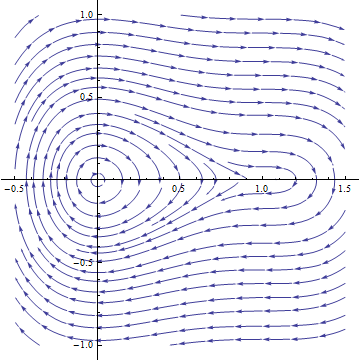
\includegraphics[scale=0.75]{./_Figures/S14Q6.png}
\end{center}

\subsubsection*{Solution to $6c$}
The ODE can be written as the system
\begin{equation}\label{s146aeq2}
\begin{aligned}
x' & = y\\
y' &= -x(1-x)^{2} - \abn{x}y.
\end{aligned}
\end{equation}
We have
$$yy' = -xy(1 - x) - |x|y^{2}$$
and hence
$$\bigg(\frac{y^{2}}{2}\bigg)' = -xx' + 2x^{2}x' - x^{3}x' - |x|y^{2} = -\bigg(\frac{x^{2}}{2}\bigg)' + \bigg(\frac{2}{3}x^{3}\bigg)' - \bigg(\frac{1}{4}x^{4}\bigg)' - |x|y^{2}.$$
Let
$$V(x, y) := \frac{y^{2}}{2} + \frac{x^{2}}{2} - \frac{2}{3}x^{3} + \frac{1}{4}x^{4}.$$
Then $V(0, 0) = 0$, $V(x, y) > 0$ for all $(x, y)$ sufficiently close to $(0, 0)$ and
$\dot{V}(x, y) = -|x|y^{2} < 0$ for all $(x, y) \neq (0, 0)$. Thus by Lyapunov theory, $(0, 0)$ is asymptotically stable.
\hfill\qed

\subsection*{Solution to Spring 2014, \#7}\label{s147}
\subsubsection*{Solution to $7a$}
We have
\begin{align*}
\dot{E}(\alpha) &= \int_{\Om}2(\Delta u + \alpha u)u\, dx\\
&= \int_{\Om}2u\delta u\, dx + 2\alpha\int_{\Om}u^{2}\, dx\\
&= -2\int_{\Om}\nabla u\cdot \nabla u\, dx + 2 \int_{\pr\Om}u\frac{\pr u}{\pr \nu}\, d\sigma + 2\alpha\int_{\Om}u^{2}\, dx\\
&= -2\int_{\Om}\nabla u \cdot \nabla u\, dx + 2 \int_{\pr\Om}u(-u)\, d\sigma + 2\alpha\int_{\Om}u^{2}\, dx
\end{align*}
where the third equality is because $u + \pr u/\pr \nu = 0$ on $\pr\Om$. Therefore as $E(r[u]) \leq E(\alpha)$ for all $\alpha \in \R$,
\begin{align*}
0 = \dot{E}(r[u]) = -2\int_{\Om}\abn{\nabla u}^{2}\, dx - 2\int_{\pr\Om}u^{2}\, d\sigma + 2r[u]\int_{\Om}u^{2}\, dx
\end{align*}
which implies
$$r[u] = \frac{\int_{\Om}\abn{\nabla u}^{2}\, dx + \int_{\pr\Om}u^{2}\, d\sigma}{\int_{\Om}u^{2}\, dx}.$$
\hfill\qed

\subsubsection*{Solution to $7b$}
Since $v$ minimizes the functional $r$ over all functions $w$ that satisfy $w(x) + \nabla w \cdot \nu = 0$ on $\pr\Om$, we must have
\begin{align}\label{s147eq1}
\frac{d}{d\vep}r[v + \vep w]\bigg|_{\vep = 0} = 0
\end{align}
for all $w$ such that $w + \nabla w \cdot \nu = 0$ on $\pr \Om$.
We compute
\begin{align*}
\bigg(\int_{\Om}&(v + \vep w)^{2}\, dx\bigg)^{2}\frac{d}{d\vep}r[v + \vep w]\\
&= \bigg(\int_{\Om}(v + \vep w)^{2}\, dx\bigg)\bigg(2\int_{\Om}\nabla(v + \vep w)\cdot \nabla w\, dx+ 2\int_{\pr\Om}(v + \vep w)w\, d\sigma\bigg)\\
&\quad\quad- \bigg(\int_{\Om}|\nabla(v + \vep w)|^{2}\, dx+ \int_{\pr\Om}(v + \vep w)^{2}\, d\sigma\bigg)\bigg(2\int_{\Om}(v + \vep w)w\, dx\bigg).
\end{align*}
Combining this with \eqref{s147eq1} yields
\begin{align*}
\bigg(\int_{\Om}v^{2}\, dx\bigg)\bigg(\int_{\Om}\nabla v \cdot \nabla w\, dx + \int_{\pr \Om}vw\, d\sigma\bigg) = \bigg(\int_{\Om}|\nabla v|^{2}\,dx + \int_{\pr\Om}v^{2}\, d\sigma\bigg)\bigg(\int_{\Om}vw\, d\sigma\bigg).
\end{align*}
Since both $v + \pr v/\pr \nu = 0$ and $w + \pr w/\pr \nu = 0$ on $\pr\Om$, integration by parts yields
$$\int_{\Om}\nabla v \cdot \nabla w\, dx = -\int_{\Om}w\Delta v\, dx - \int_{\pr\Om}wv\, d\sigma$$
and
\begin{align}\label{s147eq2}
\int_{\Om}\nabla v \cdot \nabla v\, dx = -\int_{\Om}v\Delta v\, dx - \int_{\pr\Om}v^{2}\, d\sigma.
\end{align}
Therefore
$$\bigg(\int_{\Om}v^{2}\, dx \bigg)\bigg(\int_{\Om}w\Delta v\, dx\bigg) = \bigg(\int_{\Om}v\Delta v\, dx\bigg)\bigg(\int_{\Om}vw\, dx\bigg).$$
Let $\alpha := \int_{\Om}v^{2}\, dx$ and $\beta := \int_{\Om}v\Delta v\, dx$. Then $\alpha\int_{\Om}w\Delta v\, dx = \beta\int_{\Om}vw\, dx$ and hence
$$\int_{\Om}w(\alpha \Delta v - \beta v)\, dx = 0$$
for all $w$ such that $w + \pr w/\pr\nu = 0$ on $\pr \Om$. This implies that $\alpha\Delta v - \beta v = 0$. That is,
\begin{align*}
\Delta v = \frac{\beta}{\alpha}v = \frac{\int_{\Om}v\Delta v\, dx}{\int_{\Om}v^{2}\, dx}v = -\bigg(\frac{\int_{\Om}\nabla v\cdot \nabla v\, dx + \int_{\pr\Om}v^{2}\, d\sigma}{\int_{\Om}v^{2}\, dx}\bigg)v = -r[v]v.
\end{align*}
\hfill\qed

\subsection*{Solution to Spring 2014, \#8}\label{s148}
We reserve $x_{0}$ to be used in the method of characteristics and will instead denote the $x_{0}$ in the problem statement as $\delta$.
For $\delta \in (0, 1)$, let
\begin{align*}
f(x) =
\begin{cases}
1 & \text{ if } 0 < x < \delta\\
0 & \text{ if } \delta < x < 1.
\end{cases}
\end{align*}
We follow the solution to Fall 2012, \#8. The characteristics of the PDE are given by $x = f(x_{0})t + x_{0}$ and crash immediately, so by the Rankine-Hugonito condition, the
shock curve $x = s(t)$ is given by
$$\dot{s}(t) = \frac{(1/2)\cdot 1^{2} - (1/2)\cdot 0^{2}}{1 - 0} = \frac{1}{2}$$
with initial condition $s(0) = \delta$. Therefore $s(t) = (1/2)t + \delta$ and so the shock is given by $x = \frac{1}{2}t +\delta$. We have the following picture.
\begin{center}
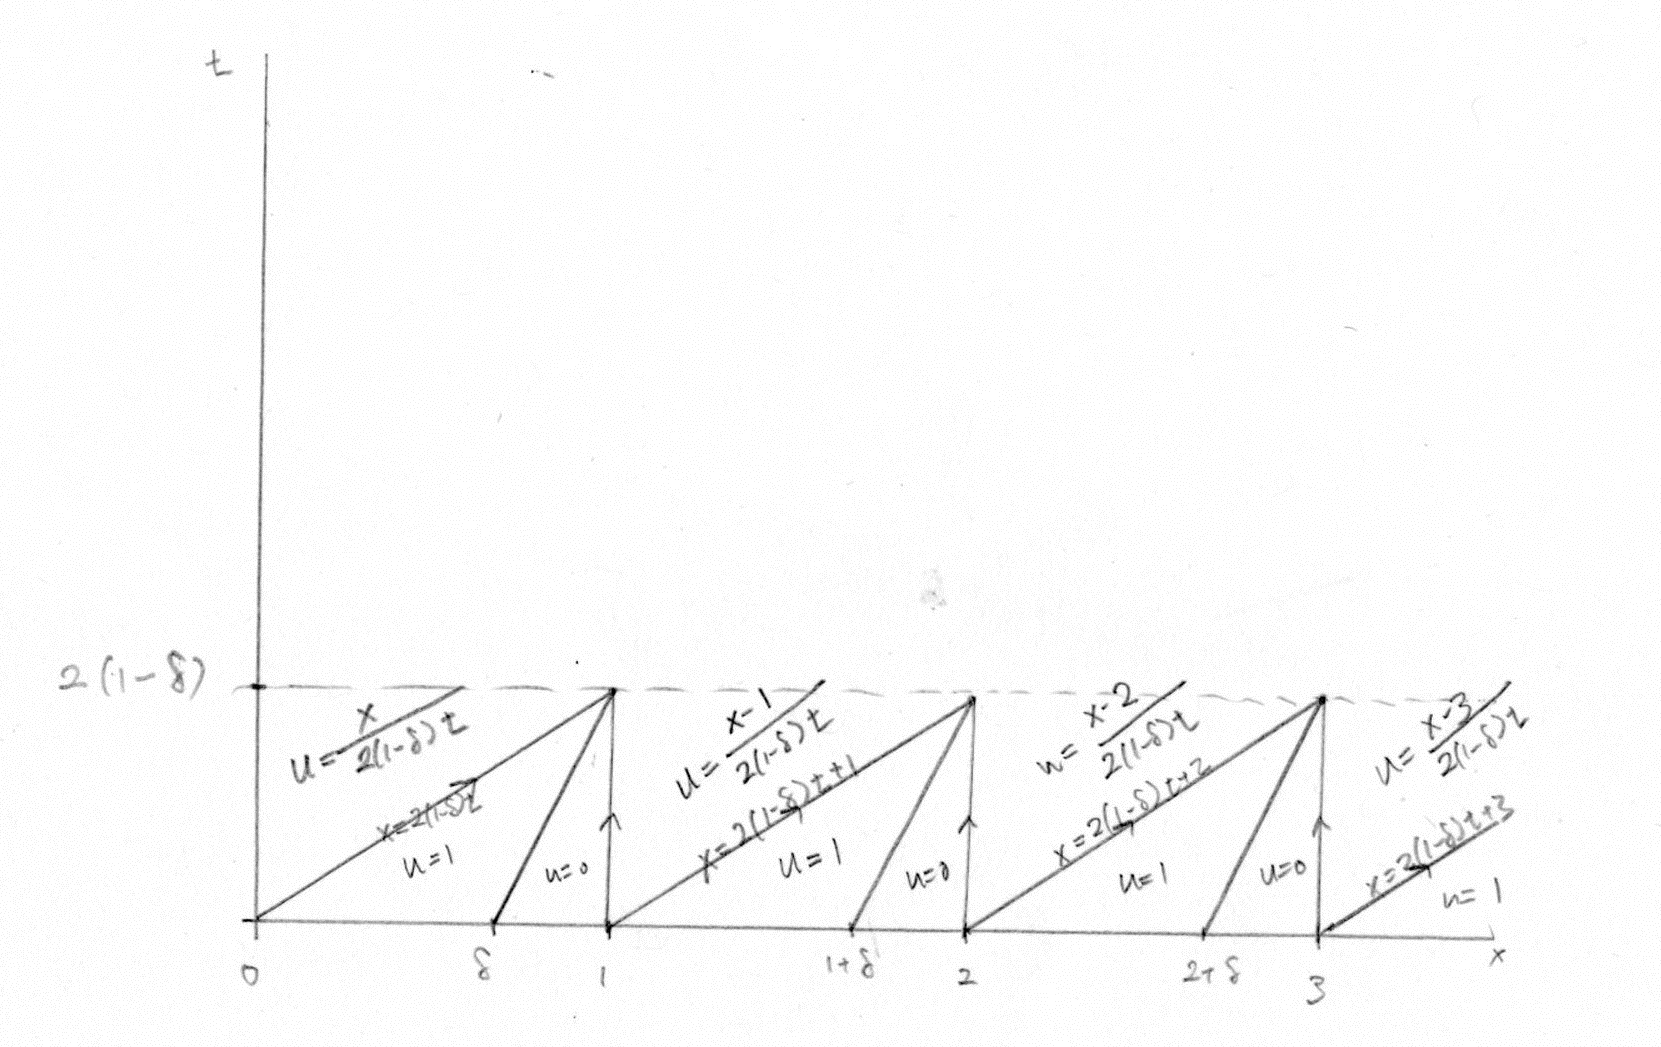
\includegraphics[scale = 0.35]{./_Figures/S14Q8a.png}
\end{center}
Thus we have another shock starting at the point $(x, t) = (k, 2(1 - \delta))$ which is given by
\begin{align*}
\dot{s}(t) = \frac{\frac{1}{2}\bigg(\frac{s(t) - (k - 1)}{2(1 - \delta)t}\bigg)^{2} - \frac{1}{2}\bigg(\frac{s(t) - k}{2(1 - \delta)t}\bigg)^{2}}{\frac{1}{2(1 - \delta)t}} = \frac{1}{2}\bigg(\frac{s(t) - k}{(1 - \delta)t} + \frac{1}{2(1 - \delta)t}\bigg) = \frac{s(t) - k + 1/2}{(1 - \delta)2t}
\end{align*}
with $s(2(1 - \delta)) = k$.
Solving this ODE via separation of variables and imposing the initial condition yields that the shock coming out of the point $(k, 2(1 - \delta))$ is given by
$$x= s(t) = \frac{1}{2}\bigg(\frac{t}{2(1 - \delta)}\bigg)^{\frac{1}{2(1 - \delta)}} + k - \frac{1}{2}.$$
Therefore the entropy solution is given by:
\begin{center}
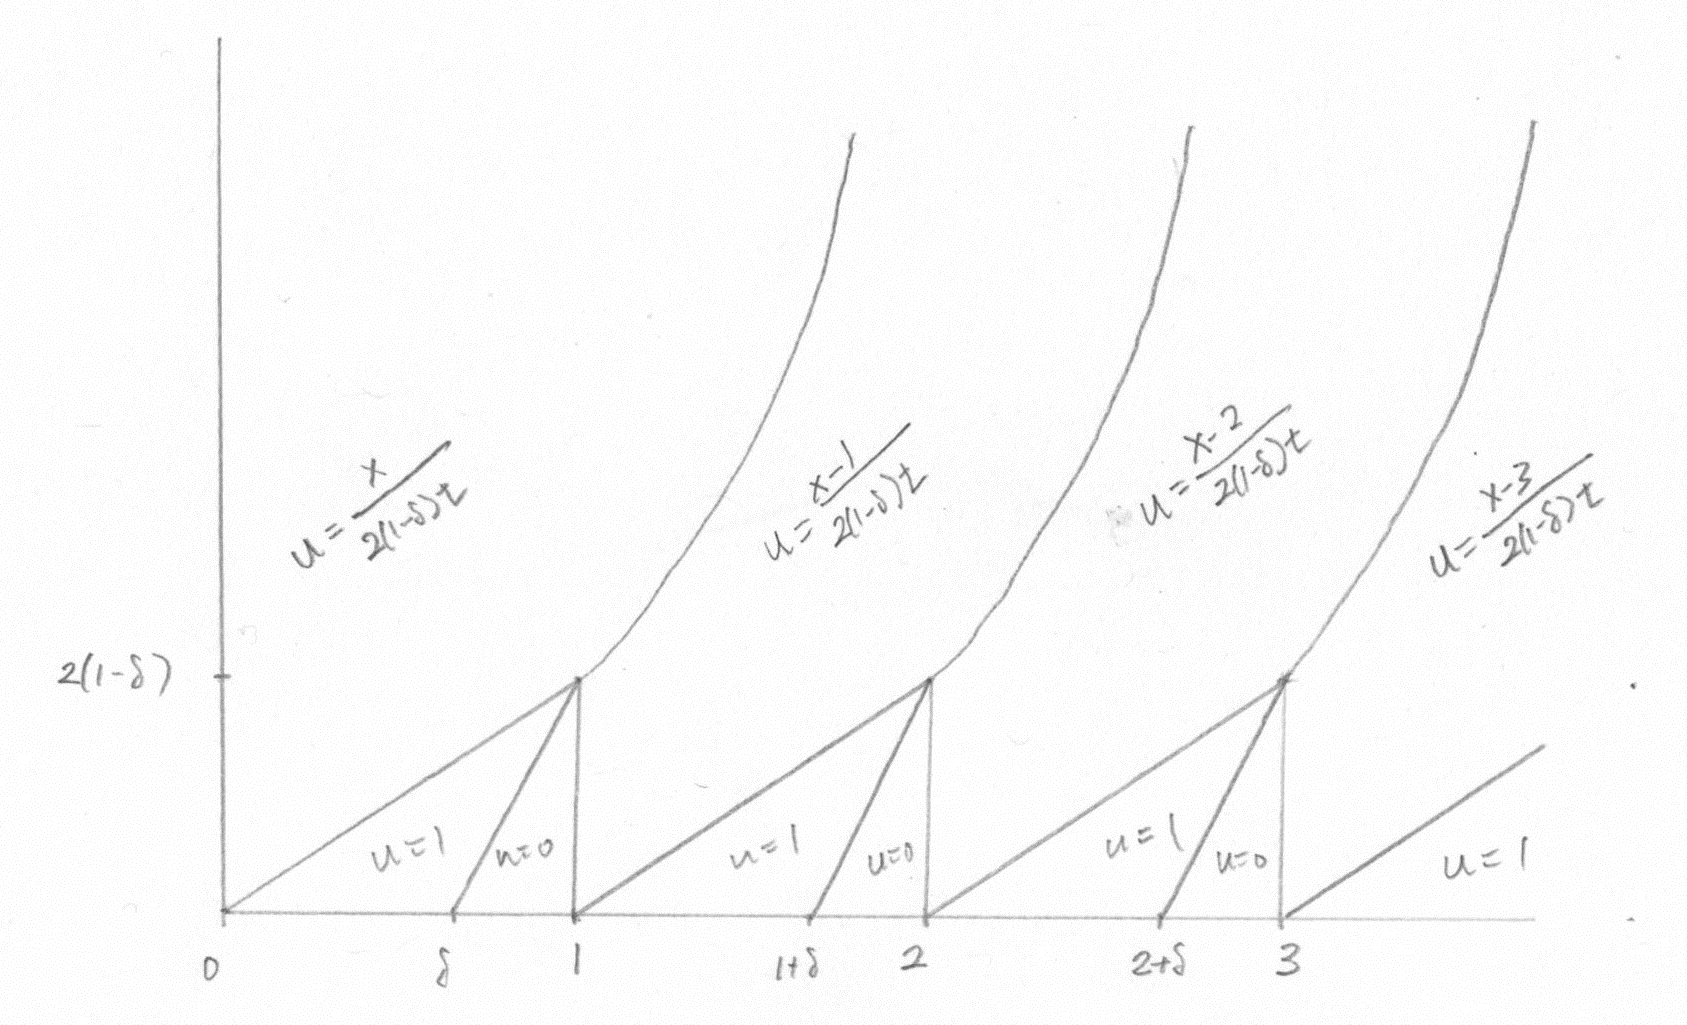
\includegraphics[scale=0.35]{./_Figures/S14Q8b.png}
\end{center}
\hfill\qed
